\documentclass[12pt,a4paper]{article}
\usepackage[utf8]{inputenc}
\usepackage[spanish]{babel}
\usepackage{graphicx}
\usepackage{kpfonts}
\usepackage[left=2cm,right=2cm,top=2cm,bottom=2cm]{geometry}
\author{Jorge Bueno}
\begin{document}
\title{Universidad Politecnica \\ de la \\ Zona Metropolitana de Guadalajara}
\author{Tarea 6\\Jorge Heriberto Bueno Gomez 18312259\\Ing. Mecatronica 4 B}
\maketitle
$$
\includegraphics[scale=.5]{UPCDLZMDG5783-logo.png} $$
\newpage
\textbf{\section{Modulación por ancho de pulsos} }
La modulación por ancho de pulsos (también conocida como PWM, siglas en inglés de pulse-width modulation) de una señal o fuente de energía es una técnica en la que se modifica el ciclo de trabajo de una señal periódica (una senoidal o una cuadrada, por ejemplo), ya sea para transmitir información a través de un canal de comunicaciones o para controlar la cantidad de energía que se envía a una carga.
El ciclo de trabajo de una señal periódica es el ancho relativo de su parte positiva en relación con el período. Expresado matemáticamente:

$$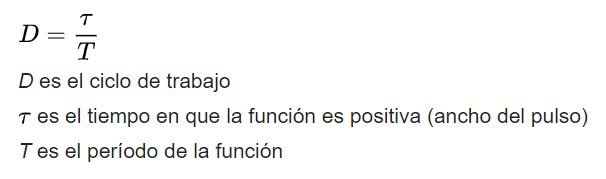
\includegraphics[scale=.5]{1.png} $$ \\
La función PWM es algo en lo que posiblemente no pensemos, un fundamento que desconoceremos si no tenemos amplios conocimientos de informática técnica, pero algo con lo que estamos más habituados de lo que podríamos imaginar. Este tipo de función se lleva a cabo en segundo plano, sin que lo sepamos, pero proporcionando ventajas importantes a nuestros equipos.

\section{Circuito usando Amp-Op y transistores}
$$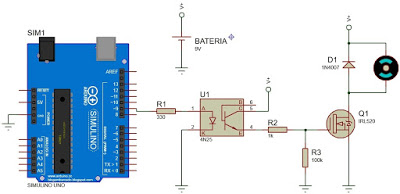
\includegraphics[scale=1]{2.jpg}$$ \\
La salida PWM- Pin (9) del Arduino  es conectada a la entrada del Optoacoplador 4n25, un dispositivo de emisión y recepción el cual funciona como un interruptor activado mediante la luz emitida por el diodo Led que satura el fototransistor, trasladando el pulso del PWM a la salida del optoacoplador. Dicho componente se utiliza para aislar electricamente el Arduino de la parte de potencia del circuito, para evitar daños en la salida del dispositivo.
La siguiente etapa consiste de un Mosfet de nivel lógico “Canal N” IRL520, en el montaje se emplean dos resistencias necesarias para el buen funcionamiento del sistema.
La resistencia de Gate (RG) limita la corriente que demanda el Gate, es decir al usar valores mas grandes de resistencias habra menor intensidad y por ende menor consumo en el Arduino, pero por otra parte si se disminuye el valor de RG favorece las transiciones más rápidas, evitando que el transistor pase menos tiempo en la zona lienal, lo que se traduce en menos temperatura en las conmutaciones es por ello que se recomienda valores habituales entre 470- 4.7K
La resistencia de Source (RS) pone el transistor a tierra (GND), cuando el pin esta en un estado indeterminado (alta impedancia), por ejemplo en el arranque del programa, se puodrian provocar encendidos y apagados del Mosfet. Un valor de resistencia de 100K a 1M llevria al Gate a tierra.


\end{document} 